\documentclass[12pt]{article}
\usepackage{graphicx}
\usepackage{amsmath}
\usepackage{hyperref}
\usepackage{float}

\title{Customer Purchase Behavior Analysis}
\author{Abdullah Yassine}
\date{Spring 2025}

\begin{document}

\maketitle

\section{Introduction}

In the age of e-commerce, understanding customer purchasing behavior is critical for businesses looking to improve product recommendations, maximize revenue, and enhance customer loyalty. Retailers thrive when they can anticipate what customers want to buy next or group customers into segments for targeted marketing. This project focuses on uncovering patterns in customer transactions through frequent itemset mining and customer segmentation techniques. The insights generated could improve real-world business strategies such as personalized marketing, product bundling, and loyalty program design.

Personally, I found this project exciting because it combines two important areas of data science — pattern mining and clustering — both of which have immediate business value. Using real transactional data to model customer behavior mirrors problems faced by modern companies like Amazon, Target, and Etsy.

\section{Data Description}

The dataset used in this project is the \textbf{Online Retail Dataset} from the \textbf{UCI Machine Learning Repository}.  
It contains approximately 541,909 rows of transactional data for a UK-based online retailer during 2010–2011.  
Each row represents a product purchased as part of a single invoice.

\subsection*{Dataset Columns}
\begin{itemize}
    \item InvoiceNo: Unique invoice number
    \item StockCode: Unique product code
    \item Description: Product description
    \item Quantity: Number of units purchased
    \item InvoiceDate: Date and time of transaction
    \item UnitPrice: Price per unit
    \item CustomerID: Unique identifier for each customer
    \item Country: Country of customer
\end{itemize}

The raw data required significant cleaning, including removing missing CustomerIDs, excluding canceled transactions (invoices starting with 'C'), and filtering out negative quantities and prices.

\section{Real-World Context}

Customer segmentation and product recommendation are key techniques widely used by companies like Amazon and Target.  
\begin{itemize}
    \item \textbf{Amazon} uses collaborative filtering to recommend products based on customer behavior.
    \item \textbf{Target} leverages purchase patterns for targeted marketing.
\end{itemize}
Academic studies such as \textit{Market Basket Analysis with Apriori Algorithm} highlight the effectiveness of association rule mining for boosting cross-sells and bundle sales.

\section{Exploratory Analysis}

Initial analysis showed certain products were extremely popular, such as \textit{WHITE HANGING HEART T-LIGHT HOLDER} and \textit{JUMBO BAG RED RETROSPOT}.

\begin{figure}[H]
    \centering
    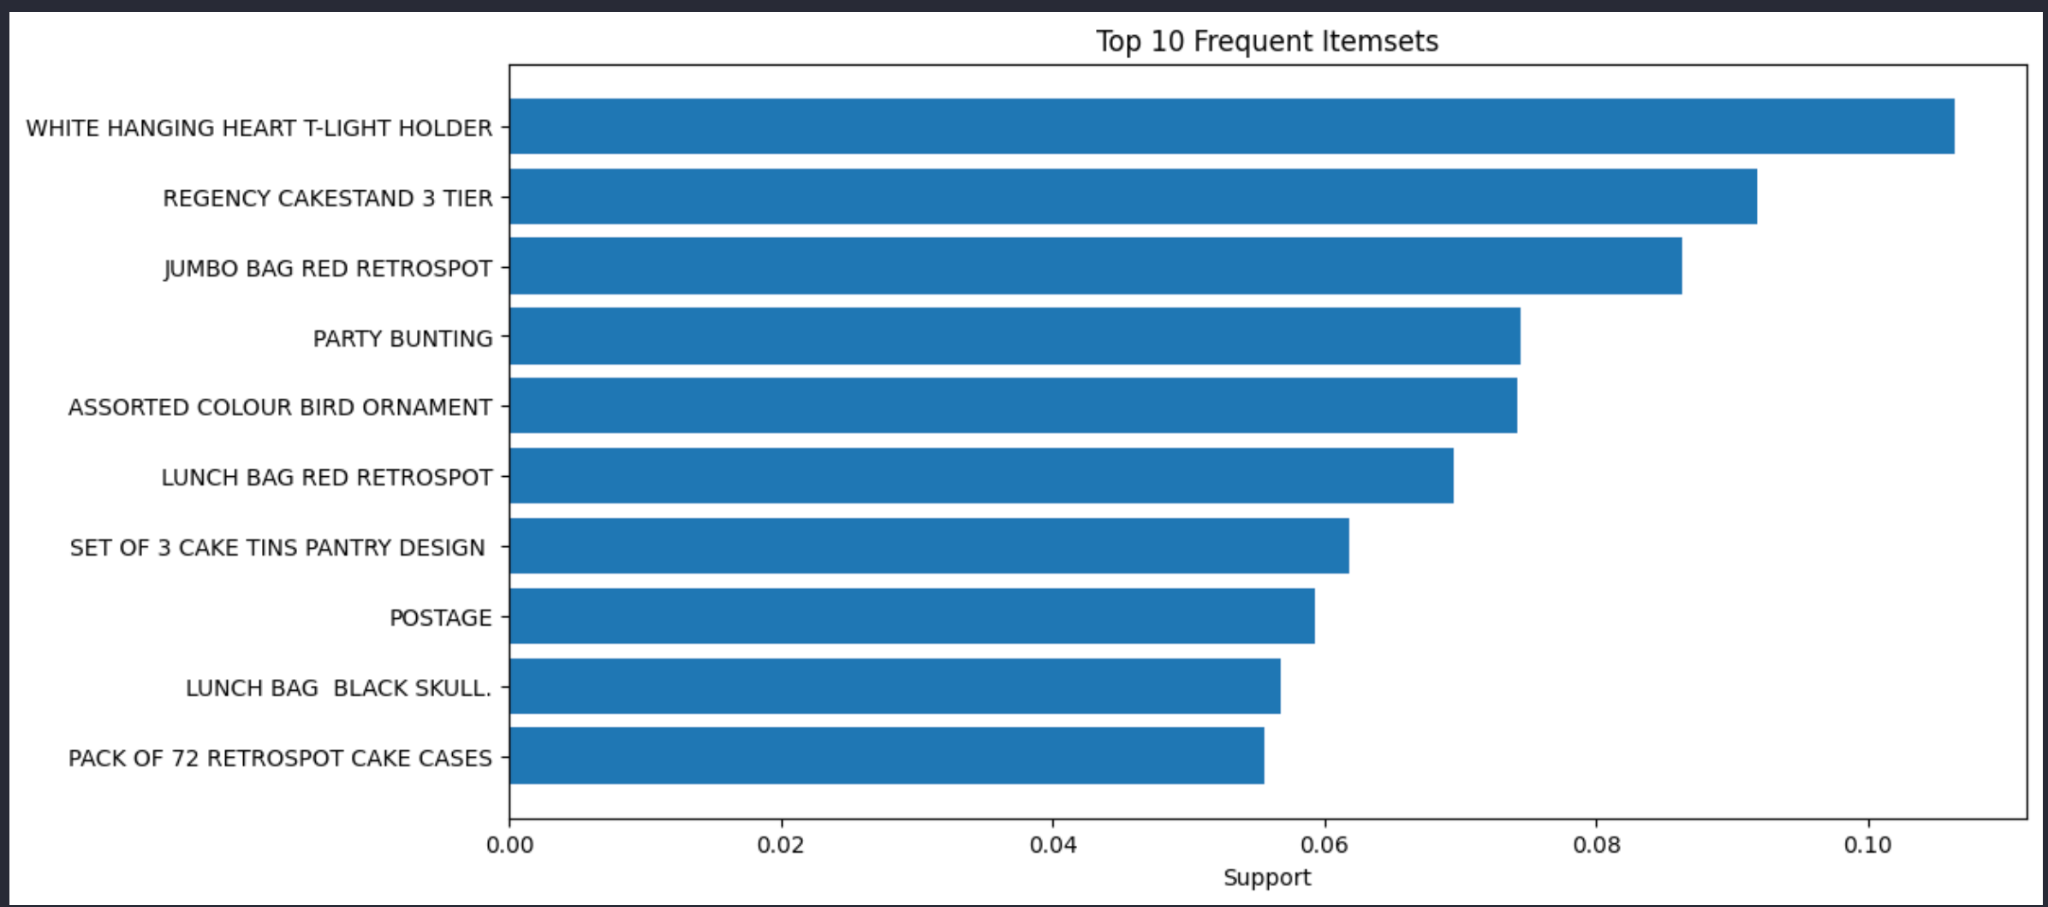
\includegraphics[width=0.7\textwidth]{images/top_10_freq_items.png}
    \caption{Top 10 Individual Products by Support}
\end{figure}

% Frequent itemsets were analyzed, showing popular co-purchases such as various lunch bags and tea cup sets.

\noindent
\textbf{Description of Figure:} \\

\vspace{0.2cm}

Figure 1 shows the \textbf{Top 10 Most Frequently Purchased Items} in the dataset, ranked by their \textit{support} values. In this context, \textbf{support} measures the proportion of all transactions that contain a given product.

\vspace{0.3cm}

\textbf{Key observations:}
\begin{itemize}
    \item \textbf{WHITE HANGING HEART T-LIGHT HOLDER} is the most purchased item, appearing in approximately 10\% of all transactions.
    \item Other highly purchased items include:
    \begin{itemize}
        \item \textit{REGENCY CAKESTAND 3 TIER}
        \item \textit{JUMBO BAG RED RETROSPOT}
        \item \textit{PARTY BUNTING}
    \end{itemize}
    \item All top 10 items have a support value greater than 5\%, indicating strong popularity across customers.
\end{itemize}

\vspace{0.3cm}

\textbf{Business implications:}
\begin{itemize}
    \item These products can be used as \textit{anchor items} in promotions or bundled offers.
    \item Inventory management should prioritize keeping these high-demand items in stock.
    \item Marketing campaigns could highlight these products to attract broader customer interest.
\end{itemize}

\vspace{0.3cm}

Overall, this plot highlights a small set of products that contribute disproportionately to sales volume. Understanding which items are consistently purchased helps businesses optimize product placement, targeted promotions, and supply chain decisions.


\begin{figure}[H]
    \centering
    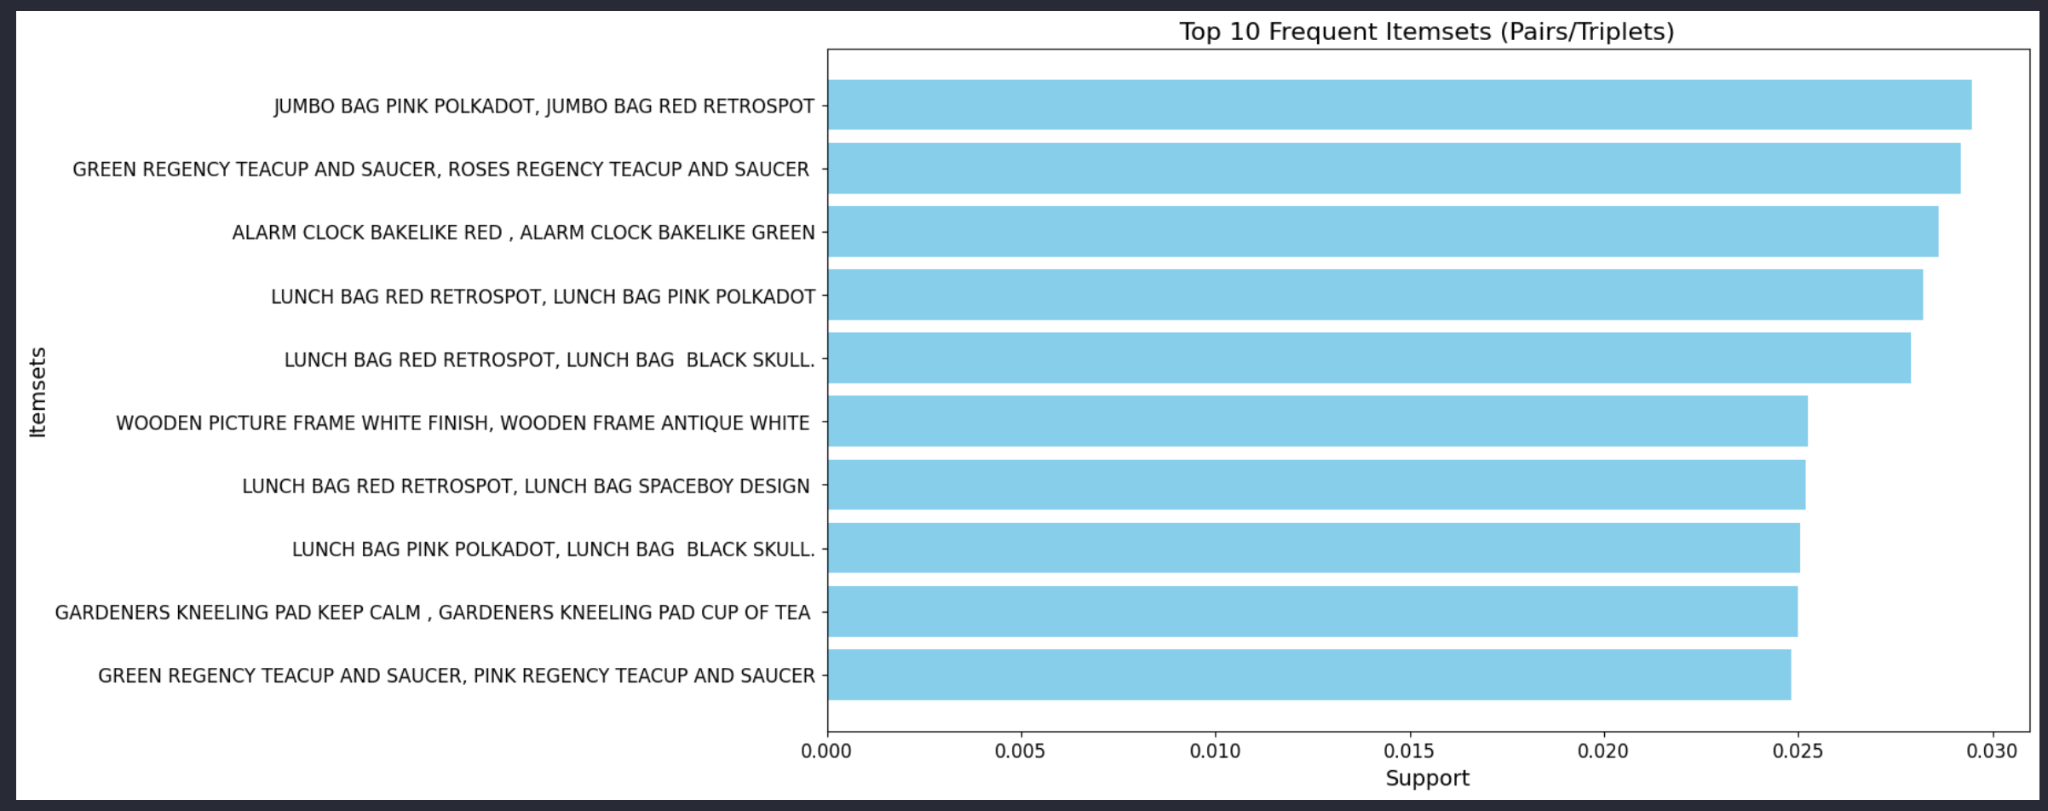
\includegraphics[width=0.7\textwidth]{images/top_10_freq_sets.png}
    \caption{Top Frequent Pairs and Triplets by Support}
\end{figure}

\noindent
\textbf{Description of Figure:} \\

\vspace{0.2cm}

Figure 2 shows the \textbf{Top 10 Most Frequent Itemsets} involving \textit{pairs} and \textit{triplets} of products.  
Here, \textbf{support} represents the proportion of all transactions that contain all items within the itemset together.

\vspace{0.4cm}

\textbf{Key observations:}
\begin{itemize}
    \item The most common co-purchased items are:
    \begin{itemize}
        \item \textit{JUMBO BAG PINK POLKADOT} and \textit{JUMBO BAG RED RETROSPOT}
        \item \textit{GREEN REGENCY TEACUP AND SAUCER} and \textit{ROSES REGENCY TEACUP AND SAUCER}
        \item \textit{ALARM CLOCK BAKELIKE RED} and \textit{ALARM CLOCK BAKELIKE GREEN}
    \end{itemize}
    \item Many of the top itemsets consist of similar or complementary products (e.g., different styles of lunch bags, matching home decor items).
    \item The support values for these itemsets are lower than individual items (as expected) but still significant, exceeding 2\%.
\end{itemize}

\vspace{0.4cm}

\textbf{Business implications:}
\begin{itemize}
    \item Bundling these frequently bought-together items could increase average cart size and revenue.
    \item Marketing strategies could suggest complementary products during checkout.
    \item Product recommendations based on these combinations would likely have high success rates, improving customer satisfaction and loyalty.
\end{itemize}

\vspace{0.4cm}

Overall, this plot reveals natural groupings of products that customers tend to purchase together, offering valuable guidance for bundling, cross-selling, and promotion strategies.


\section{Methods}

\subsection{Frequent Itemset Mining}

The Apriori algorithm was used with a minimum support threshold of 2\%.  
Association rules were generated where lift was greater than 1.  
Apriori is efficient because it expands itemsets level by level, pruning combinations that are not frequent early on.

\subsection{Customer Segmentation}

RFM features were engineered:
\begin{itemize}
    \item Recency: Days since last purchase
    \item Frequency: Number of purchases
    \item Monetary: Total amount spent
\end{itemize}

Features were standardized, and clustering was performed using:
\begin{itemize}
    \item \textbf{K-Means Clustering} (hard assignment)
    \item \textbf{Gaussian Mixture Models (GMM)} (soft probabilistic assignment)
\end{itemize}

\subsection{Gaussian Mixture Model Formula}

The probability model for GMM is:

\[
p(x) = \sum_{k=1}^{K} \phi_k \mathcal{N}(x | \mu_k, \Sigma_k)
\]

where:
\begin{itemize}
    \item \( \phi_k \) are mixing coefficients
    \item \( \mu_k \) are mean vectors
    \item \( \Sigma_k \) are covariance matrices
\end{itemize}

\section{Results}

\subsection{Frequent Itemsets and Rules}

Customers frequently bought:
\begin{itemize}
    \item Multiple lunch bags (different styles)
    \item Matching tea cups and saucers
    \item Bundles of reusable shopping bags
\end{itemize}

\begin{figure}[H]
    \centering
    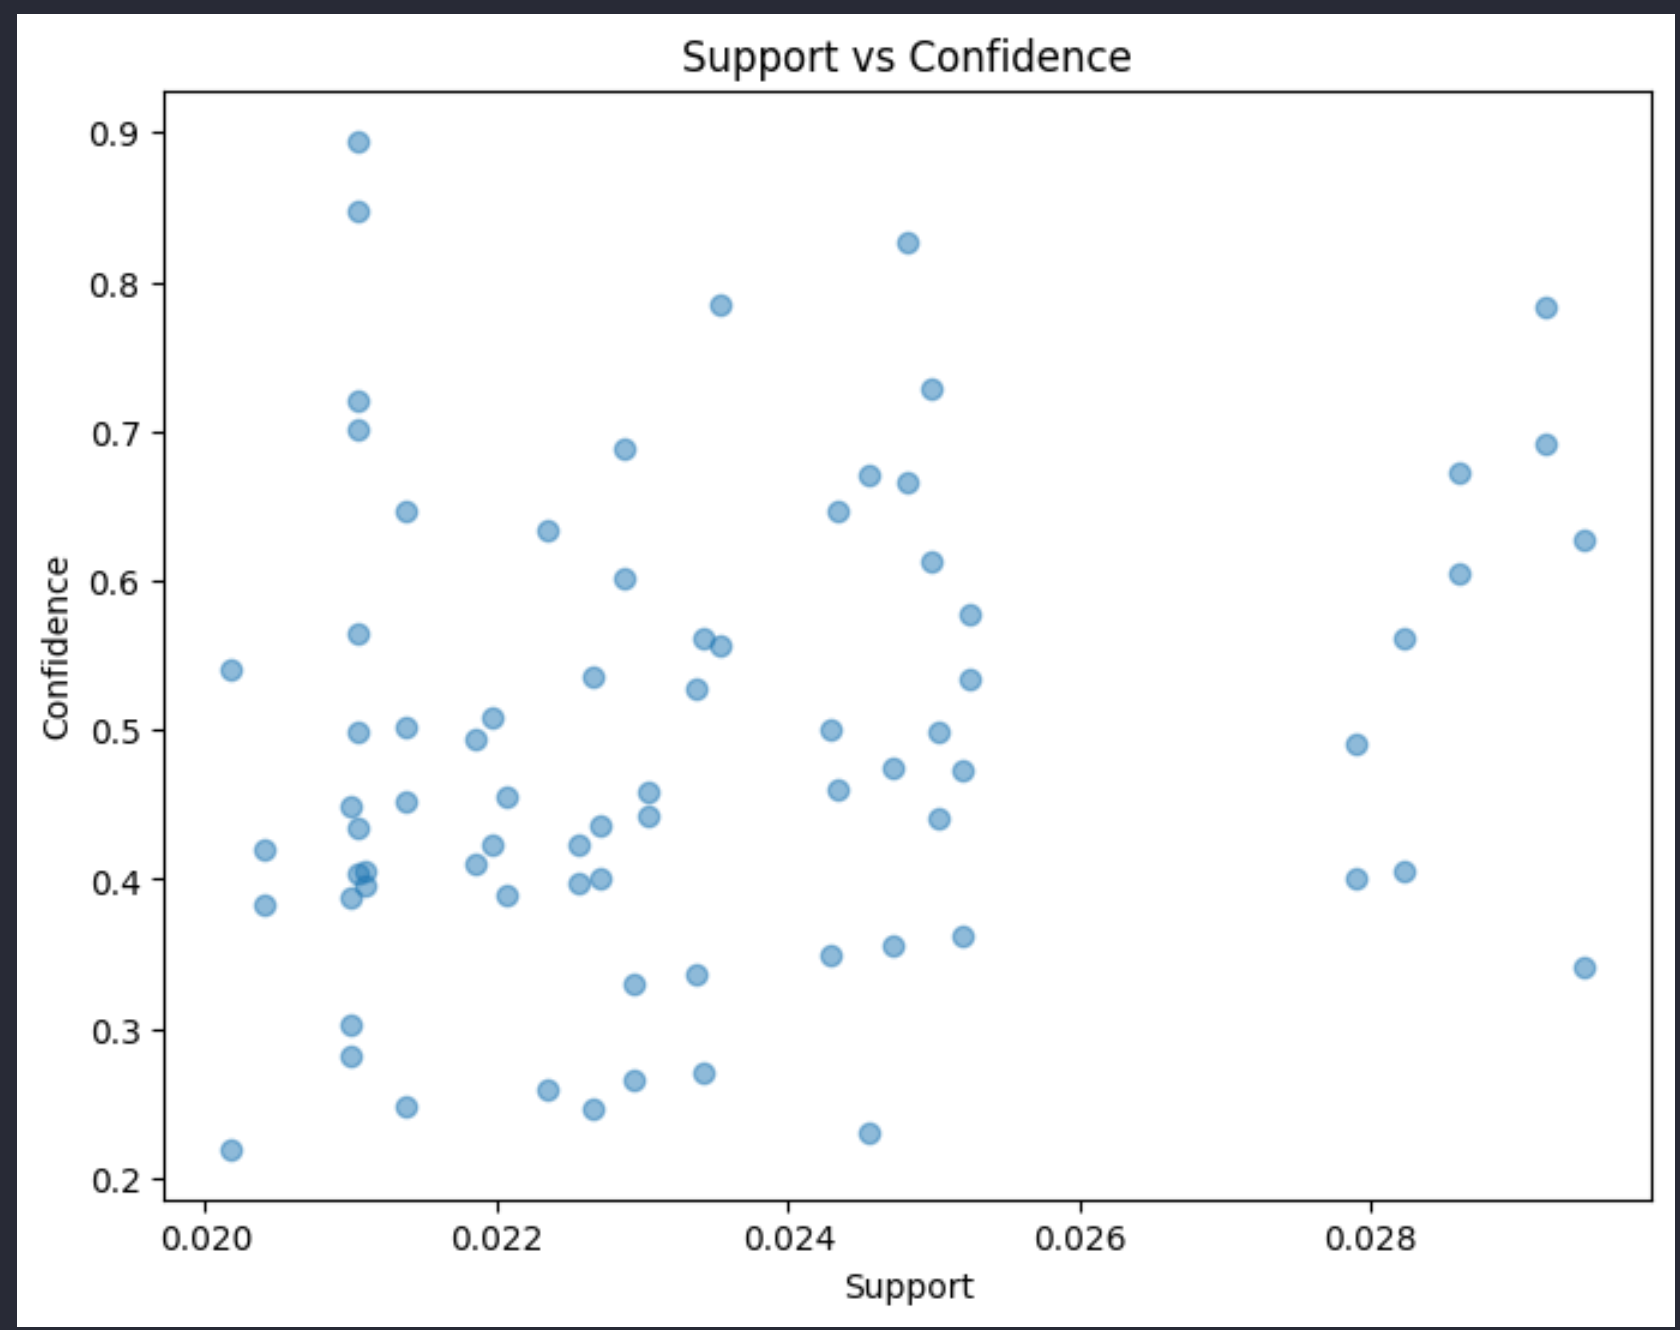
\includegraphics[width=0.7\textwidth]{images/support_vs_confidence.png}
    \caption{Association Rules: Support vs Confidence}
\end{figure}

\noindent
\textbf{Description of Figure:} \\

\vspace{0.2cm}

Figure 3 presents a \textbf{scatter plot of Support versus Confidence} for the association rules generated from frequent itemsets.  
Each point on the graph represents a single association rule between items.

\vspace{0.4cm}

\textbf{Understanding the axes:}
\begin{itemize}
    \item \textbf{Support (x-axis):}  
    The proportion of all transactions that contain both the antecedent and consequent items.  
    Higher support values indicate that the rule involves more commonly purchased items.
    
    \item \textbf{Confidence (y-axis):}  
    The probability that a transaction containing the antecedent item(s) also contains the consequent item(s).  
    Higher confidence means the rule is more reliable for making predictions.
\end{itemize}

\vspace{0.4cm}

\textbf{Key observations:}
\begin{itemize}
    \item Most rules have support values ranging between 0.02 and 0.03, meaning they apply to 2\%–3\% of all transactions.
    \item Confidence values are more widely spread, ranging from 0.2 to over 0.9.
    \item There is no obvious linear relationship between support and confidence. Some rules have high confidence but relatively low support, indicating they are very reliable but occur less frequently.
    \item Densely packed points around confidence 0.4–0.5 suggest that many rules have moderate reliability.
\end{itemize}

\vspace{0.4cm}

\textbf{Business implications:}
\begin{itemize}
    \item High-confidence rules, even with moderate support, are valuable for personalized recommendations because they represent strong purchasing patterns.
    \item Rules with both high support and high confidence are ideal candidates for automated marketing strategies such as "Frequently Bought Together" promotions.
    \item Understanding the trade-off between support and confidence helps businesses balance between recommending highly reliable rules versus more popular item combinations.
\end{itemize}

\vspace{0.4cm}

Overall, this plot provides a comprehensive view of the reliability and prevalence of various product association rules, enabling better decision-making for recommendation systems and targeted offers.


\subsection{Customer Segmentation: KMeans Clusters}

\begin{figure}[H]
    \centering
    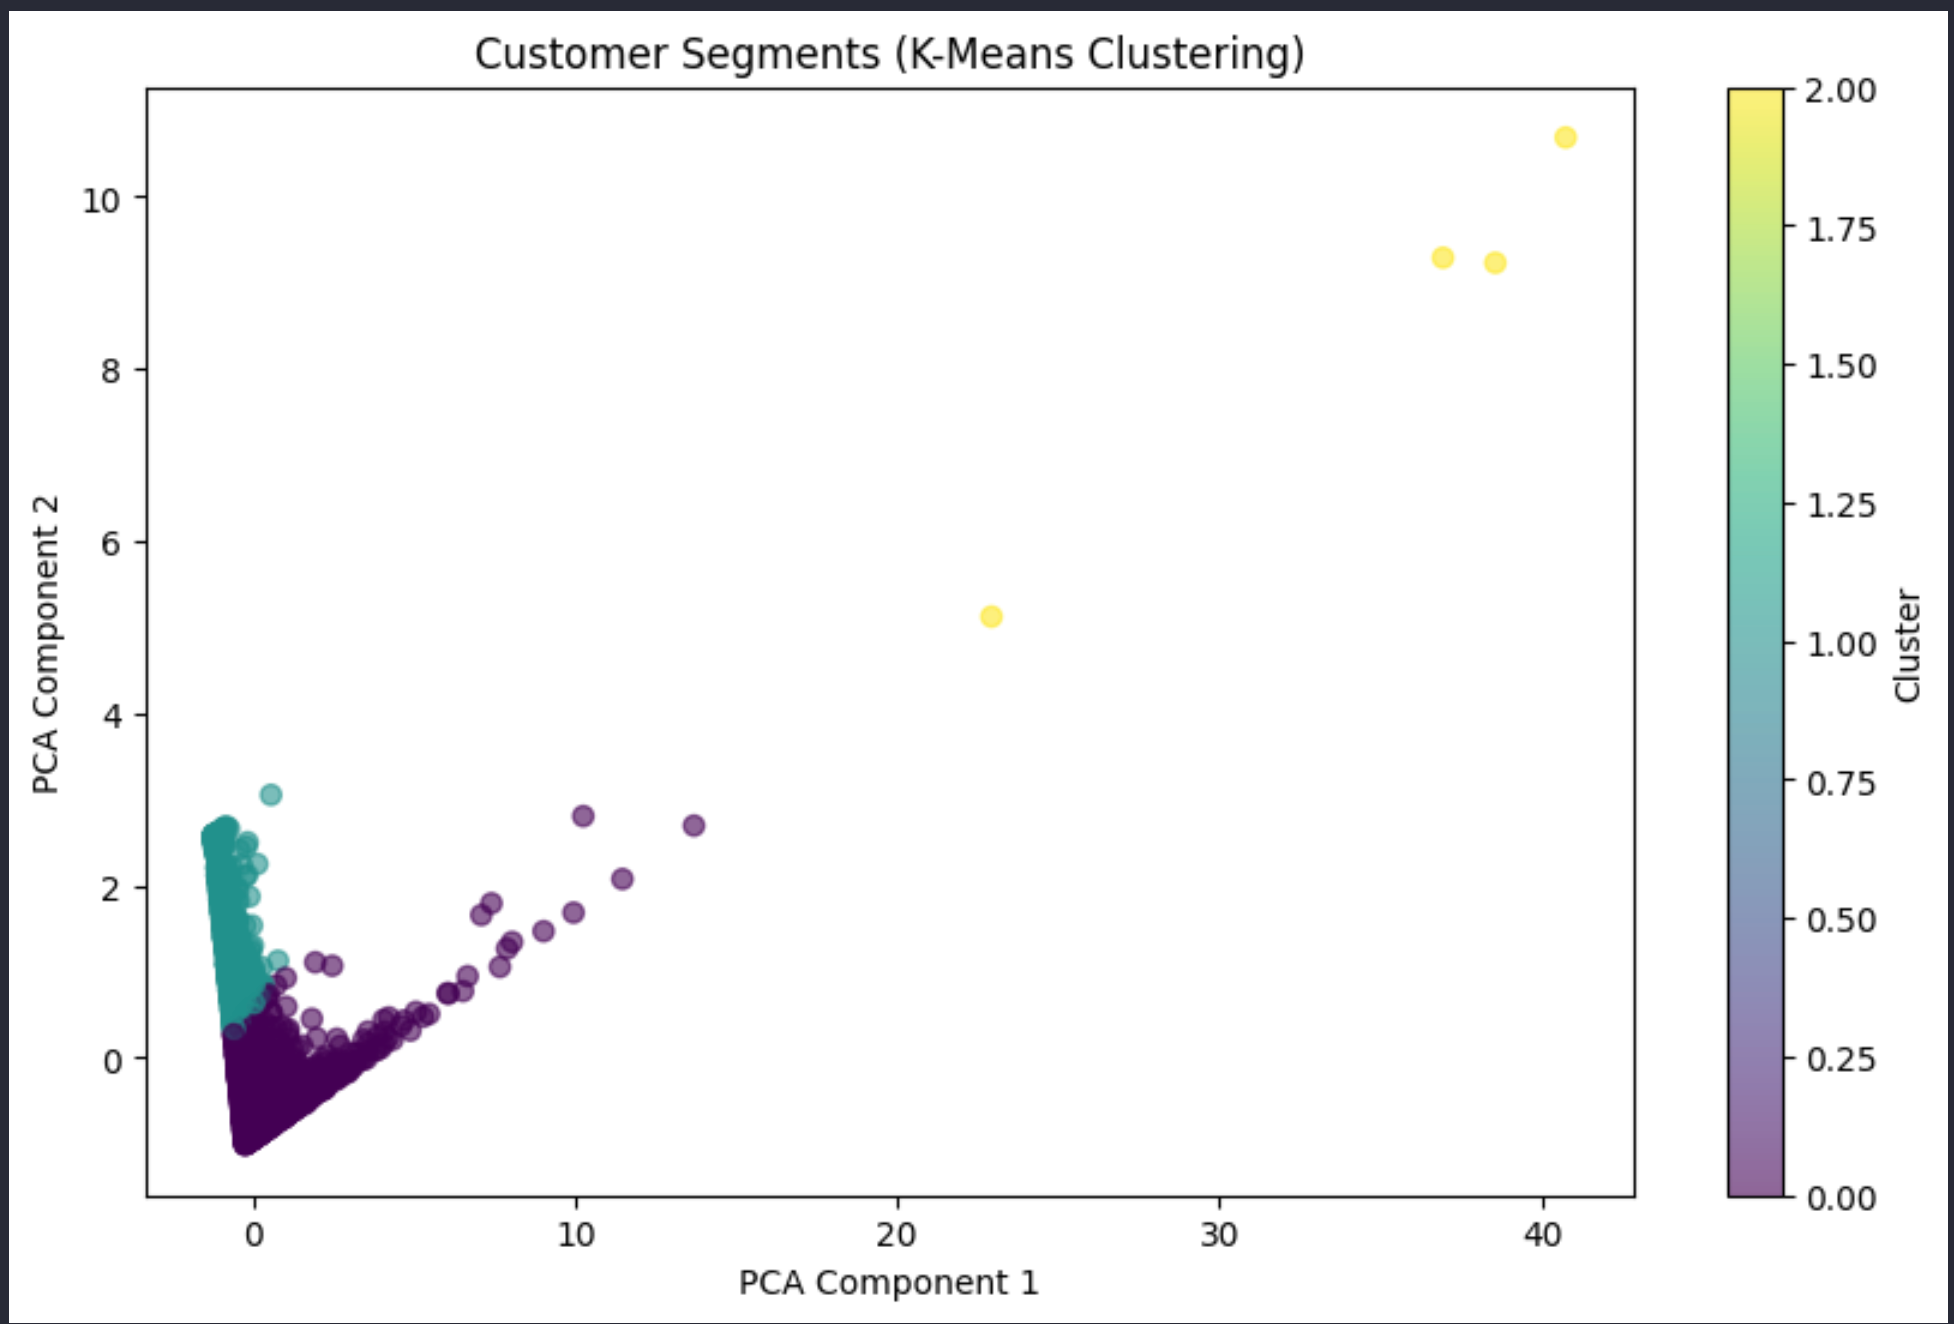
\includegraphics[width=0.7\textwidth]{images/customer_clusters_k_means.png}
    \caption{KMeans Customer Clusters (PCA Projection)}
\end{figure}

\noindent
\textbf{Description of Figure:} \\

\vspace{0.2cm}

Figure 4 shows the \textbf{K-Means Clustering Results} visualized using a \textbf{2D Principal Component Analysis (PCA) projection}.  
Each point represents a customer, colored according to the cluster assignment determined by the K-Means algorithm.

\vspace{0.4cm}

\textbf{Understanding the axes:}
\begin{itemize}
    \item \textbf{PCA Component 1} and \textbf{PCA Component 2} are synthetic features created by PCA to capture the maximum variance in the original three-dimensional RFM data (Recency, Frequency, Monetary).
    \item These components are linear combinations of the original features and allow for easier 2D visualization while preserving the general structure of the data.
\end{itemize}

\vspace{0.4cm}

\textbf{Key observations:}
\begin{itemize}
    \item Three distinct clusters are visible, suggesting that customers naturally group into three main behavioral segments.
    \item The yellow cluster (Cluster 2) is noticeably separated, representing customers who are very different from the majority. These could be extremely high-value buyers (very frequent purchases, high spending).
    \item The dark purple and teal clusters (Clusters 0 and 1) represent customers who are closer together but still distinct in terms of their purchasing patterns.
    \item Some customers (points) are more spread out, indicating variability even within clusters, while most customers are densely packed near the center.
\end{itemize}

\vspace{0.4cm}

\textbf{Business implications:}
\begin{itemize}
    \item The identification of clear clusters allows businesses to create tailored marketing strategies:
    \begin{itemize}
        \item High-value customers (yellow cluster) can be targeted with loyalty rewards and premium offers.
        \item Moderate customers can be encouraged to spend more through promotions.
        \item Low-engagement customers could receive reactivation campaigns or targeted discounts.
    \end{itemize}
    \item Understanding how customers group naturally helps prioritize marketing budget and resources effectively.
\end{itemize}

\vspace{0.4cm}

Overall, this plot demonstrates that customer behavior is not random but forms structured patterns that businesses can leverage to drive personalized engagement and improve lifetime value.

\vspace{0.4cm}


\textbf{KMeans Clusters Summary:}
\begin{itemize}
    \item Cluster 2: Super buyers (extremely high frequency and monetary)
    \item Cluster 0: Loyal customers (good frequency and spending)
    \item Cluster 1: At-risk customers (long recency, low frequency)
\end{itemize}

\subsection{Customer Segmentation: GMM Clusters}

\begin{figure}[H]
    \centering
    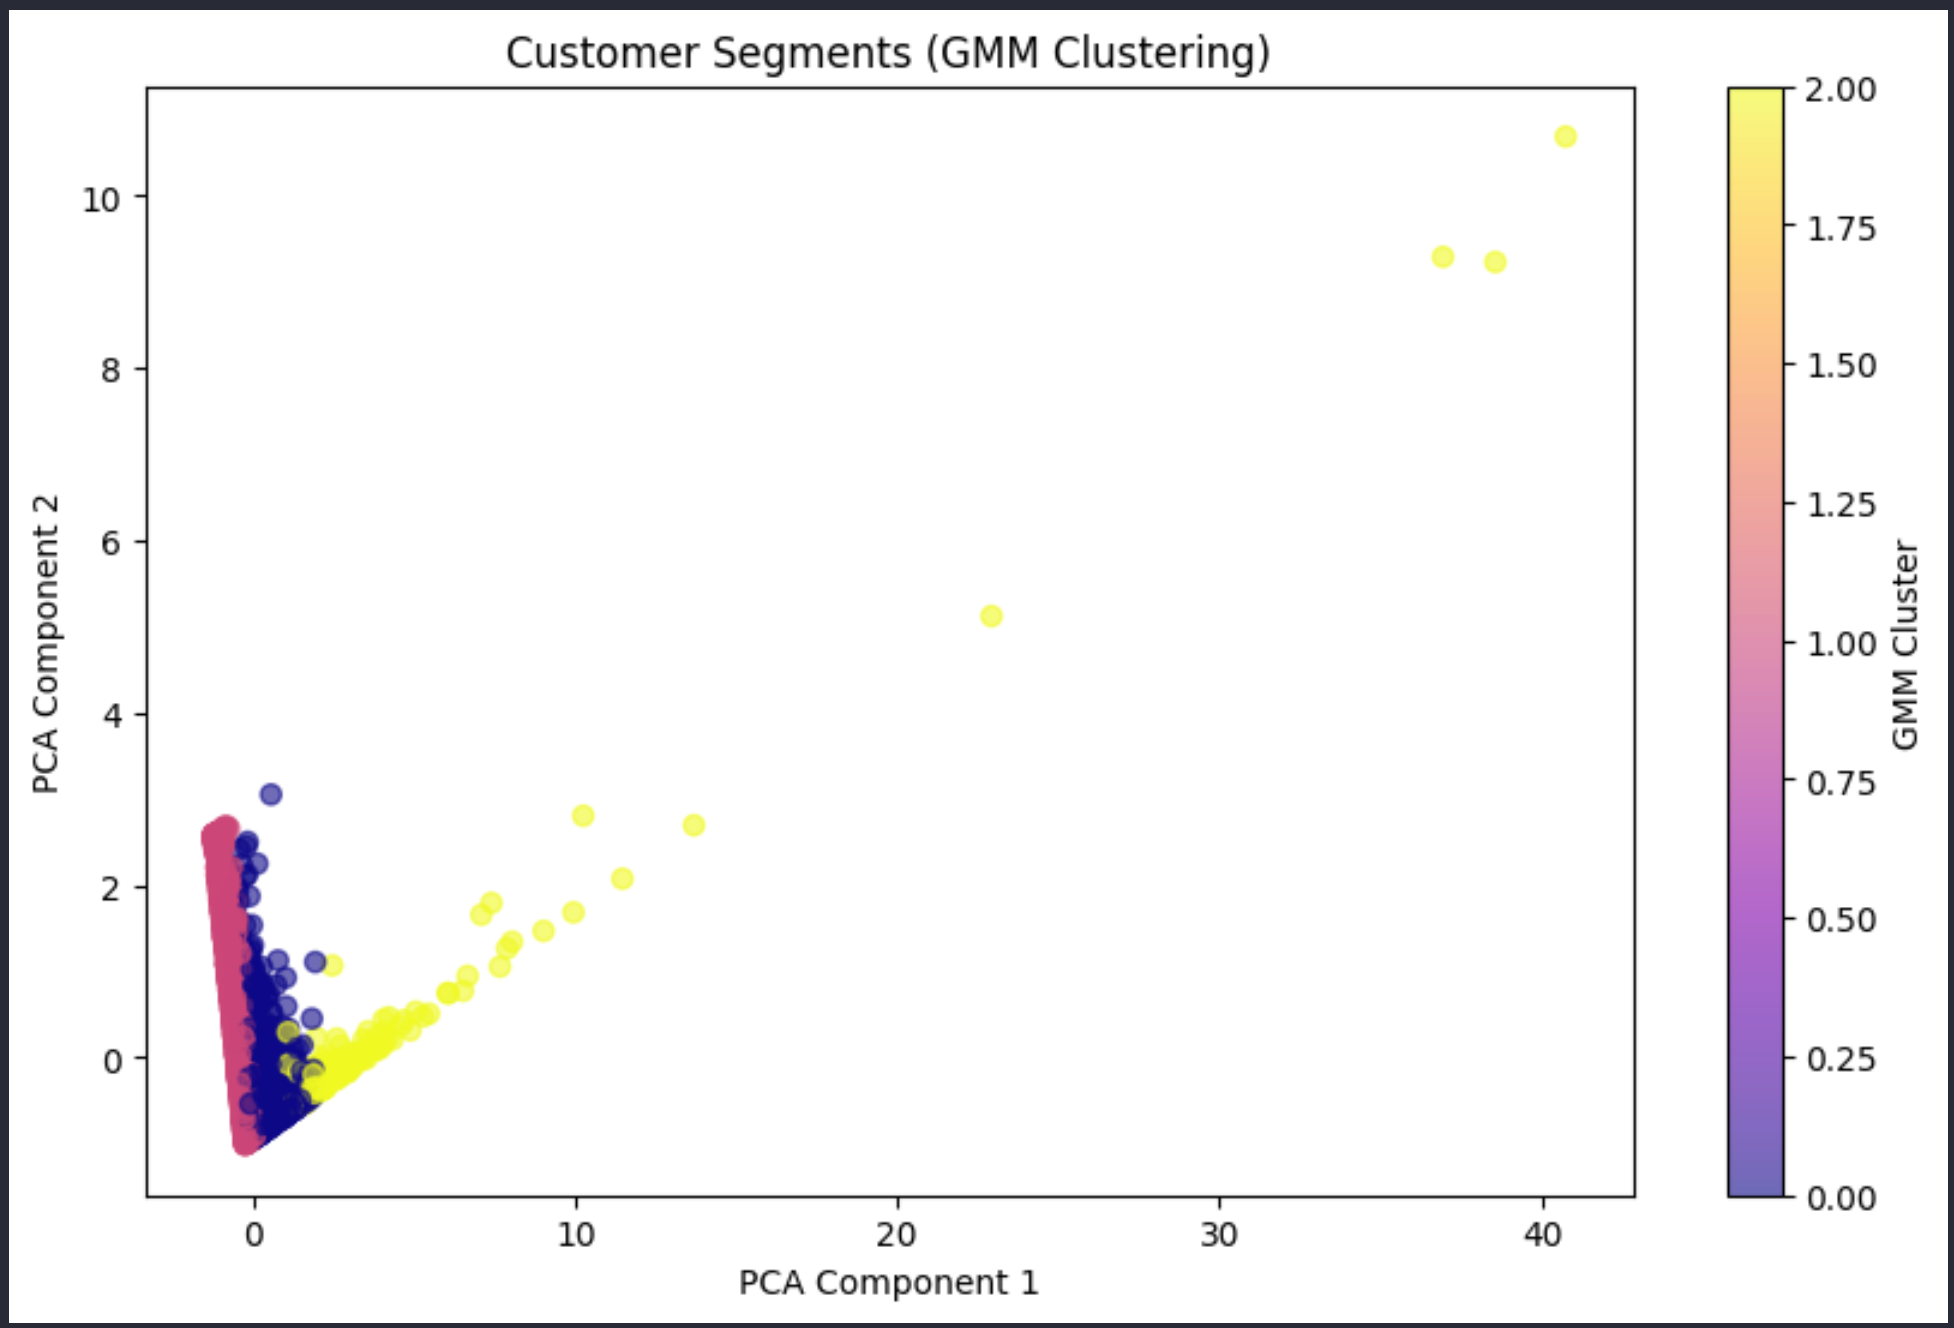
\includegraphics[width=0.7\textwidth]{images/customers_clusters_gmm_clustering.png}
    \caption{GMM Customer Clusters (PCA Projection)}
\end{figure}

\noindent
\textbf{Description of Figure:} \\

\vspace{0.2cm}

Figure 5 displays the \textbf{Gaussian Mixture Model (GMM) Clustering Results} visualized using a \textbf{2D PCA projection}.  
Each point represents a customer, colored by their GMM-assigned cluster membership based on Recency, Frequency, and Monetary (RFM) features.

\vspace{0.4cm}

\textbf{Understanding the axes:}
\begin{itemize}
    \item \textbf{PCA Component 1} and \textbf{PCA Component 2} are principal components derived from the original RFM variables.
    \item These components summarize the variation in customer behavior into two dimensions, making it possible to visualize customer groupings in 2D.
\end{itemize}

\vspace{0.4cm}

\textbf{Understanding GMM clustering:}
\begin{itemize}
    \item Unlike K-Means, where each customer belongs to exactly one cluster, GMM assigns customers a probability of belonging to each cluster.
    \item Customers near the boundaries between clusters might have a high probability for multiple clusters, resulting in softer or overlapping cluster boundaries.
\end{itemize}

\vspace{0.4cm}

\textbf{Key observations:}
\begin{itemize}
    \item Three main clusters are identified, matching the number found through K-Means, confirming the natural structure of the data.
    \item The yellow-colored cluster (Cluster 2) consists of customers that are extreme in purchasing behavior — possibly super-buyers or very high-frequency purchasers.
    \item The darker clusters (Clusters 0 and 1) represent the majority of customers, but some overlap is more visible compared to the K-Means result, showing how customer behavior is sometimes mixed between groups.
    \item There are a few highly dispersed points, indicating customers whose behavior deviates significantly from the general population.
\end{itemize}

\vspace{0.4cm}

\textbf{Business implications:}
\begin{itemize}
    \item GMM clustering provides a probabilistic view of customer segmentation, allowing businesses to handle "in-between" customers more flexibly.
    \item Customers with split probabilities between clusters could receive mixed marketing strategies tailored to their diverse behaviors.
    \item Identifying the distinct super-buyer cluster helps focus loyalty programs and premium offerings on the most valuable customers.
\end{itemize}

\vspace{0.4cm}

Overall, this GMM clustering visualization demonstrates that customer purchasing behavior follows underlying patterns but is not strictly divided.  
Soft clustering allows for more nuanced and flexible customer engagement strategies in real-world business applications.

\vspace{0.4cm}


GMM clustering produced similar findings to KMeans, confirming the customer segments' robustness.

\section{Conclusion}

This project successfully applied frequent itemset mining and customer clustering techniques to extract valuable insights from e-commerce transactional data.  
Through the Apriori algorithm, we identified strong product associations, such as bundles of lunch bags and coordinated home decor items.  
Clustering customers based on Recency, Frequency, and Monetary (RFM) behavior revealed distinct customer segments: \textbf{super-buyers}, \textbf{loyal regulars}, and \textbf{at-risk customers}.

\vspace{0.4cm}

\textbf{Key Takeaways:}
\begin{itemize}
    \item \textbf{Frequent itemset mining} highlights cross-sell and bundle opportunities that could immediately boost revenue and improve customer satisfaction.
    \item \textbf{Customer segmentation} provides a foundation for more effective marketing campaigns, allowing businesses to tailor promotions based on customer value and engagement level.
    \item The combination of market basket analysis and RFM clustering demonstrates how traditional data science methods can deliver actionable business strategies.
\end{itemize}

\vspace{0.4cm}

\subsection*{Potential Future Work}

Looking ahead, several extensions could deepen the business and data science impact:

\begin{itemize}
    \item \textbf{Seasonality Analysis:}  
    Investigate how purchasing patterns vary across seasons, holidays, or sales events, enabling time-sensitive promotions.
    
    \item \textbf{Predictive Customer Churn Modeling:}  
    Build classification models (e.g., Logistic Regression, Random Forests, XGBoost) to predict which customers are at risk of leaving, allowing proactive re-engagement strategies.
    
    \item \textbf{Dynamic Recommendation Systems:}  
    Move beyond frequent itemsets by implementing more sophisticated recommendation models such as Collaborative Filtering, Matrix Factorization, or Neural Network-based recommendation engines.
    
    \item \textbf{Customer Lifetime Value (CLV) Modeling:}  
    Estimate the future value of a customer using regression or survival analysis models to optimize long-term marketing investment.
    
    \item \textbf{Deep Learning for Pattern Discovery:}  
    Use autoencoders or embedding techniques (e.g., Word2Vec for products) to uncover hidden structures in purchase behavior beyond simple item combinations.
\end{itemize}

\vspace{0.4cm}

\textbf{Final Thoughts:}  
By better understanding customer behavior and purchasing relationships, businesses can personalize the customer experience, increase customer retention, and drive sustainable revenue growth.  
Integrating more advanced machine learning models would allow for even more precise, dynamic, and scalable insights, ensuring businesses stay competitive in the rapidly evolving world of digital commerce.

\end{document}
